% !TEX root = ../main.tex

% 结语部分
\section{APL1-4 电子自旋共振实验 \\ The End}


%---------------------------------------------------------------------
% 总结、杂谈与致谢
\subsection{Summary, Thoughts \& Acknowledgments}
\begin{enumerate}
	\item Thank you, teacher, for taking the time to read this experimental report, which still has many shortcomings. I hope you can point out the areas that need improvement. I wish you good health, happiness in life, and success in your work!
\end{enumerate}


%---------------------------------------------------------------------
% 附件
\subsection{Attachment}
The arrangement of the experimental bench desktop is shown in %\cref{}.

The personal signature of the experimental report is shown in \cref{fig:name}.

\begin{figure}[htbp]
	\centering
	
\includegraphics[width=0.6\textwidth]{name.png}
	\caption{signature}
	\label{fig:name}
\end{figure}

\textbf{All relevant code (Python and LaTex source code) has been uploaded to Github.}

\subsection{Schedule}

\begin{figure}[h!]
	\centering
	\caption{【实验1】数据记录表（记录人\&时间：\hspace{4cm}）}
	\label{fig:apl14exp1tab}
	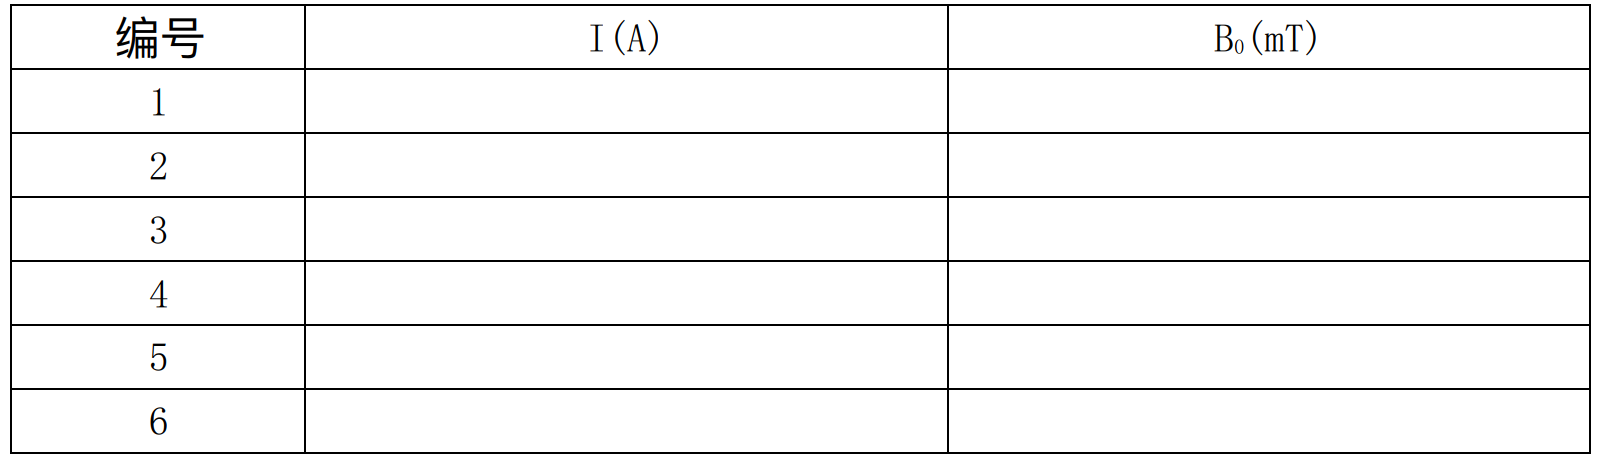
\includegraphics[width=0.9\linewidth]{images/APL1_4_exp1_tab}
\end{figure}

\begin{table}[h!]
	\centering
	\caption{【实验2】数据记录表（记录人\&时间：\hspace{4cm}）}
	\renewcommand{\arraystretch}{1.5}
	\begin{tabular}{|c|c|c|c|c|c|}
		\hline
		\textbf{序号} & \textbf{励磁电源电压 (V)} & \textbf{磁感应强度 $B$ (G)} & \textbf{微波频率 $f$ (GHz)} & \textbf{示波器信号强度} & \textbf{朗德因子 $g$} \\ \hline
		1 & \hspace{3cm} & \hspace{2.5cm} & \hspace{2.5cm} & \hspace{2.5cm} & \hspace{2.5cm} \\ \hline
		2 & \hspace{3cm} & \hspace{2.5cm} & \hspace{2.5cm} & \hspace{2.5cm} & \hspace{2.5cm} \\ \hline
		3 & \hspace{3cm} & \hspace{2.5cm} & \hspace{2.5cm} & \hspace{2.5cm} & \hspace{2.5cm} \\ \hline
		4 & \hspace{3cm} & \hspace{2.5cm} & \hspace{2.5cm} & \hspace{2.5cm} & \hspace{2.5cm} \\ \hline
		5 & \hspace{3cm} & \hspace{2.5cm} & \hspace{2.5cm} & \hspace{2.5cm} & \hspace{2.5cm} \\ \hline
	\end{tabular}
\end{table}

\begin{table}[h!]
	\centering
	\caption{【实验3】数据记录表（记录人\&时间：\hspace{4cm}）}
	\renewcommand{\arraystretch}{1.5}
	\begin{tabular}{|c|c|c|c|c|c|c|}
		\hline
		\textbf{序号} & \textbf{扫场相位} & \textbf{共振峰重合} & \textbf{半高宽 $\Delta t$ (s)} & \textbf{扫场幅度 $B'$ (G)} & \textbf{横向弛豫时间 $T_2$ (s)} & \textbf{备注} \\ \hline
		1 & \hspace{2cm} & \hspace{2.5cm} & \hspace{2.5cm} & \hspace{2.5cm} & \hspace{2.5cm} & \hspace{1cm} \\ \hline
		2 & \hspace{2cm} & \hspace{2.5cm} & \hspace{2.5cm} & \hspace{2.5cm} & \hspace{2.5cm} & \hspace{1cm} \\ \hline
		3 & \hspace{2cm} & \hspace{2.5cm} & \hspace{2.5cm} & \hspace{2.5cm} & \hspace{2.5cm} & \hspace{1cm} \\ \hline
		4 & \hspace{2cm} & \hspace{2.5cm} & \hspace{2.5cm} & \hspace{2.5cm} & \hspace{2.5cm} & \hspace{1cm} \\ \hline
		5 & \hspace{2cm} & \hspace{2.5cm} & \hspace{2.5cm} & \hspace{2.5cm} & \hspace{2.5cm} & \hspace{1cm} \\ \hline
	\end{tabular}
\end{table}

\begin{table}[h!]
	\centering
	\caption{【实验4】数据记录表（记录人\&时间：\hspace{4cm}）}
	\renewcommand{\arraystretch}{1.5}
	\begin{tabular}{|c|c|c|c|c|}
		\hline
		\textbf{序号} & \textbf{谐振点位置 $L_1$ (cm)} & \textbf{谐振点位置 $L_2$ (cm)} & \textbf{谐振点位置 $L_3$ (cm)} & \textbf{波导波长 $\lambda_g$ (cm)} \\ \hline
		1 & \hspace{3cm} & \hspace{3cm} & \hspace{3cm} & \hspace{3cm} \\ \hline
		2 & \hspace{3cm} & \hspace{3cm} & \hspace{3cm} & \hspace{3cm} \\ \hline
		3 & \hspace{3cm} & \hspace{3cm} & \hspace{3cm} & \hspace{3cm} \\ \hline
		4 & \hspace{3cm} & \hspace{3cm} & \hspace{3cm} & \hspace{3cm} \\ \hline
		5 & \hspace{3cm} & \hspace{3cm} & \hspace{3cm} & \hspace{3cm} \\ \hline
	\end{tabular}
\end{table}

%---------------------------------------------------------------------
% 参考文献
\renewcommand{\refname}{Reference}
\begin{thebibliography}{99}	
	\bibitem{a} 维基百科. \emph{维基百科}[M]. https://zh.wikipedia.org
	\bibitem{b} 沈韩. \emph{基础物理实验}[M]. 北京: 科学出版社, 2015.	
\end{thebibliography}